\chapter[Simulatie resultaten DCF]{Simulatieresultaten van het DCF77 blok}
\label{Ap: dcf_sim}
\phantomsection\subsection*{\refstepcounter{subsection}\label{fig: edge_beh}\thesubsection.\quad Behaviour edge detector}
\begin{figure}[ht!]
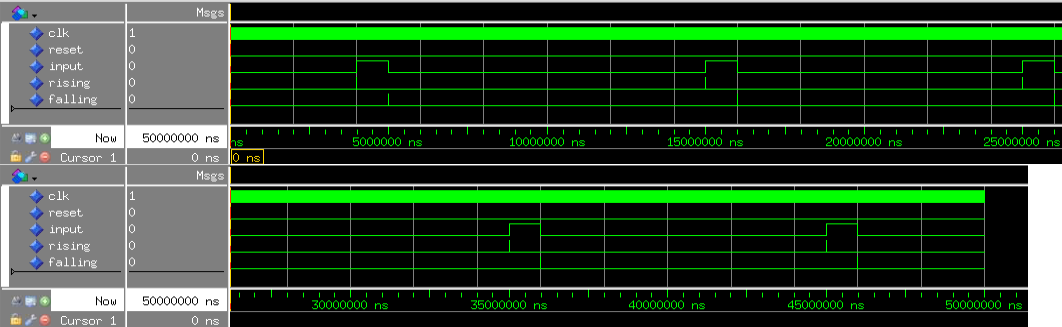
\includegraphics[width=\textwidth,height=\textheight,keepaspectratio]{Figuren/DCF77/Edge_detector.png}
\caption{Simulatie van de edge detector (50 ms op schaal)}
\end{figure}
\phantomsection\subsection*{\refstepcounter{subsection}\label{fig: count_beh}\thesubsection.\quad Behaviour DCF counter}
\begin{figure}[ht!]
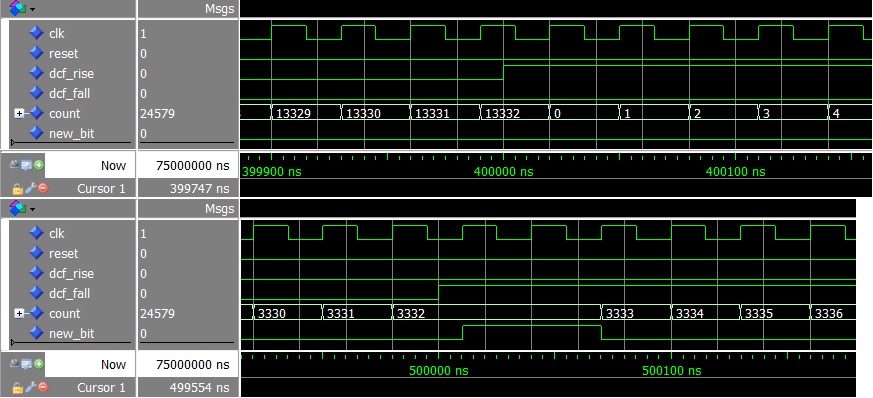
\includegraphics[width=\textwidth,height=\textheight,keepaspectratio]{Figuren/DCF77/Counter.png}
\caption{Simulatie van de DCF counter (details van 75 ms op schaal)}
\end{figure}
\phantomsection\subsection*{\refstepcounter{subsection}\label{fig: decoder_beh}\thesubsection.\quad Behaviour DCF decoder}
\begin{figure}[ht!]
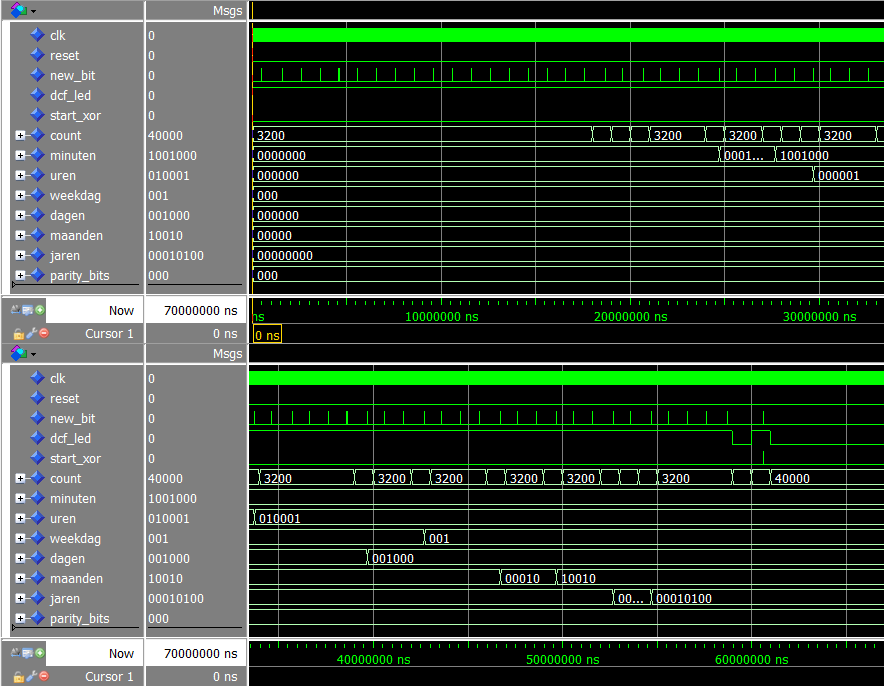
\includegraphics[width=\textwidth,height=\textheight,keepaspectratio]{Figuren/DCF77/Decoder.png}
\caption{Simulatie van de DCF decoder (70 ms op schaal)}
\end{figure}
\phantomsection\subsection*{\refstepcounter{subsection}\label{fig: parity_beh}\thesubsection.\quad Behaviour parity check}
\begin{figure}[ht!]
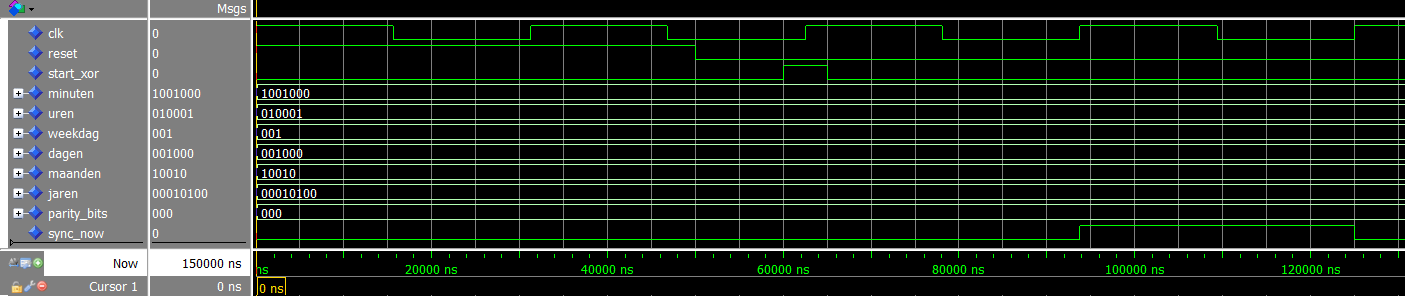
\includegraphics[width=\textwidth,height=\textheight,keepaspectratio]{Figuren/DCF77/Parity_check.png}
\caption{Simulatie van de parity check (150 microseconden)}
\end{figure}
\phantomsection\subsection*{\refstepcounter{subsection}\label{fig: synctime_beh}\thesubsection.\quad Behaviour synctime}
\begin{figure}[ht!]
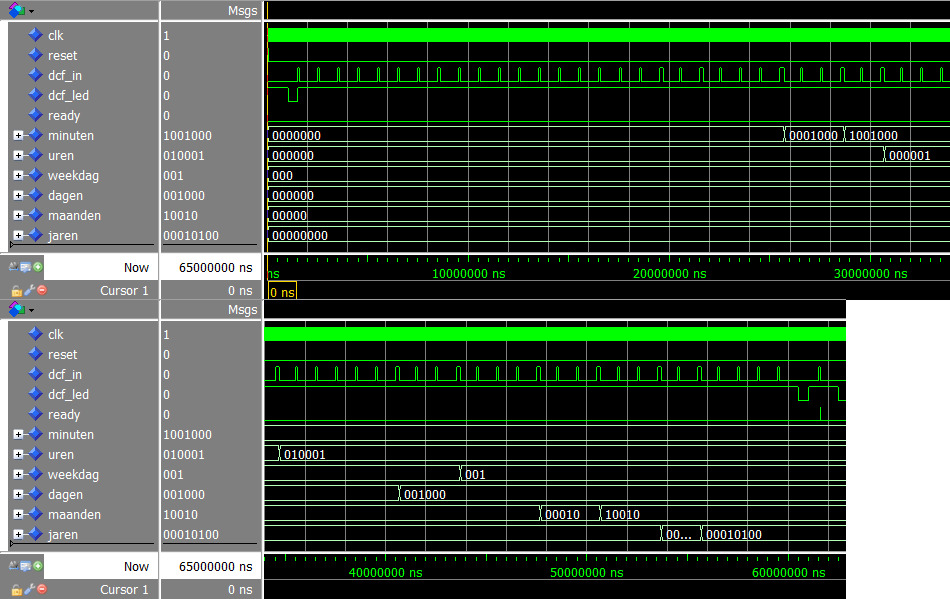
\includegraphics[width=\textwidth,height=\textheight,keepaspectratio]{Figuren/DCF77/Synctime.png}
\caption{Simulatie van synctime (65 ms op schaal)}
\end{figure}
\phantomsection\subsection*{\refstepcounter{subsection}\label{fig: klokdeler_beh}\thesubsection.\quad Behaviour klokdeler}
\begin{figure}[ht!]
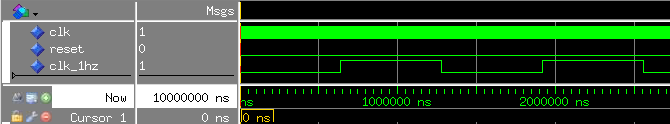
\includegraphics[width=\textwidth,height=\textheight,keepaspectratio]{Figuren/DCF77/Klokdeler.png}
\caption{Simulatie van de  klokdeler (10 ms op schaal)}
\end{figure}
\phantomsection\subsection*{\refstepcounter{subsection}\label{fig: mod24_beh}\thesubsection.\quad Behaviour mod24 teller}
\begin{figure}[ht!]
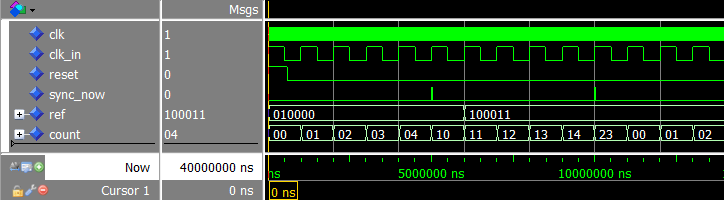
\includegraphics[width=\textwidth,height=\textheight,keepaspectratio]{Figuren/DCF77/Mod24_teller.png}
\caption{Simulatie van de mod24 teller (40 ms op schaal)}
\end{figure}
\phantomsection\subsection*{\refstepcounter{subsection}\label{fig: mod601_beh}\thesubsection.\quad Behaviour mod60 teller}
\begin{figure}[ht!]
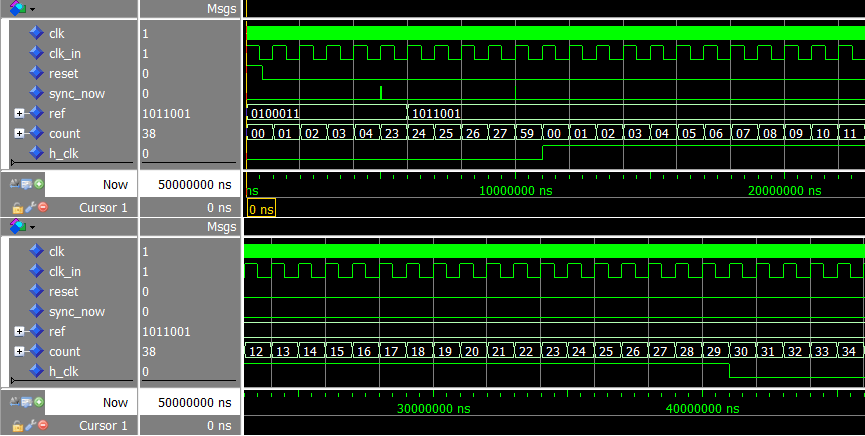
\includegraphics[width=\textwidth,height=\textheight,keepaspectratio]{Figuren/DCF77/Mod60_teller.png}
\caption{Simulatie van de mod60 teller (50 ms op schaal)}
\end{figure}
\phantomsection\subsection*{\refstepcounter{subsection}\label{fig: mod602_beh}\thesubsection.\quad Behaviour mod60 clock}
\begin{figure}[ht!]
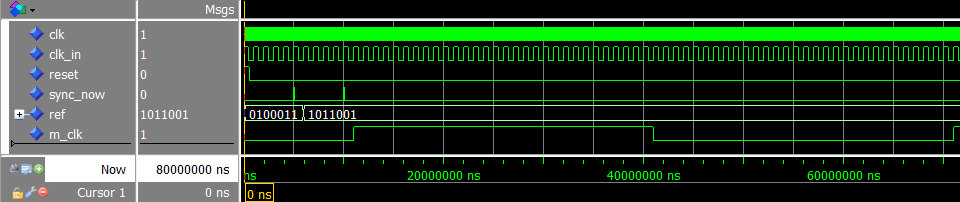
\includegraphics[width=\textwidth,height=\textheight,keepaspectratio]{Figuren/DCF77/Mod60_clock.png}
\caption{Simulatie van de mod60 clock (80 ms op schaal)}
\end{figure}
\phantomsection\subsection*{\refstepcounter{subsection}\label{fig: klok_beh}\thesubsection.\quad Behaviour klok}
\begin{figure}[ht!]
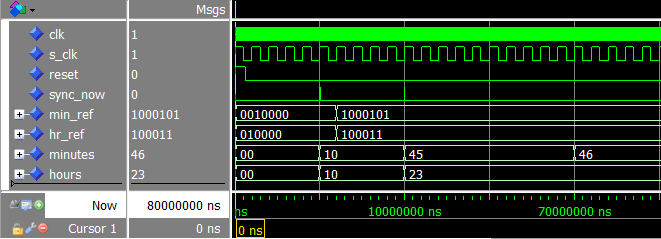
\includegraphics[width=\textwidth,height=\textheight,keepaspectratio]{Figuren/DCF77/Klok.png}
\caption{Simulatie van de klok (80 ms op schaal)}
\end{figure}
\phantomsection\subsection*{\refstepcounter{subsection}\label{fig: beh}\thesubsection.\quad Behaviour DCF77 blok}
\begin{figure}[ht!]
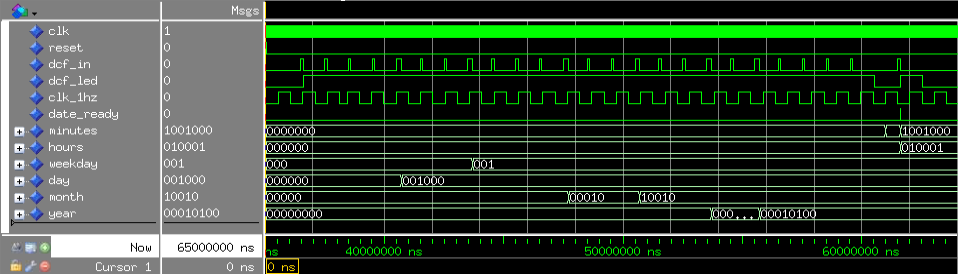
\includegraphics[width=\textwidth,height=\textheight,keepaspectratio]{Figuren/DCF77/Behaviour.png}
\caption{Simulatie van het DCF77 blok (65 ms op schaal)}
\end{figure}
\phantomsection\subsection*{\refstepcounter{subsection}\label{fig: switchlevel}\thesubsection.\quad Switch-level DCF77 blok}
\begin{figure}[ht!]
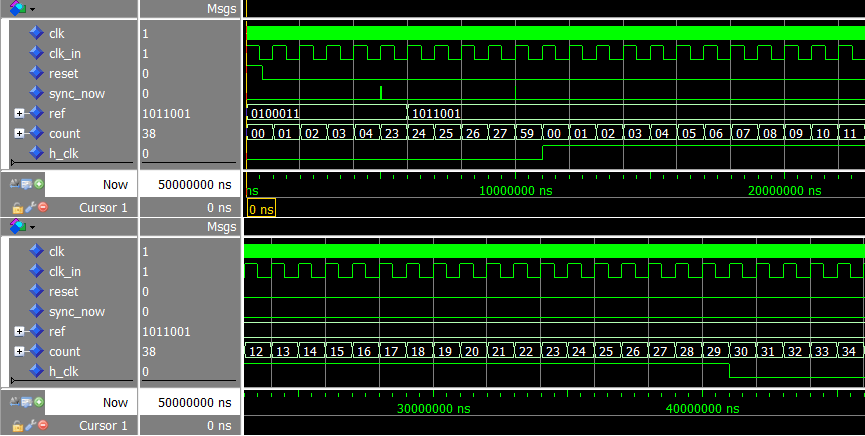
\includegraphics[width=\textwidth,height=\textheight,keepaspectratio]{Figuren/DCF77/Mod60_teller.png}
\caption{Switch-level simulatie van het DCF77 blok (65 ms op schaal)}
\end{figure}


\chapter[Simulatie resultaten]{Simulaties resultaten van de controller}
\label{Ap:sim_controller}
\section{Behavioral simulatie}
\begin{figure}[ht!]
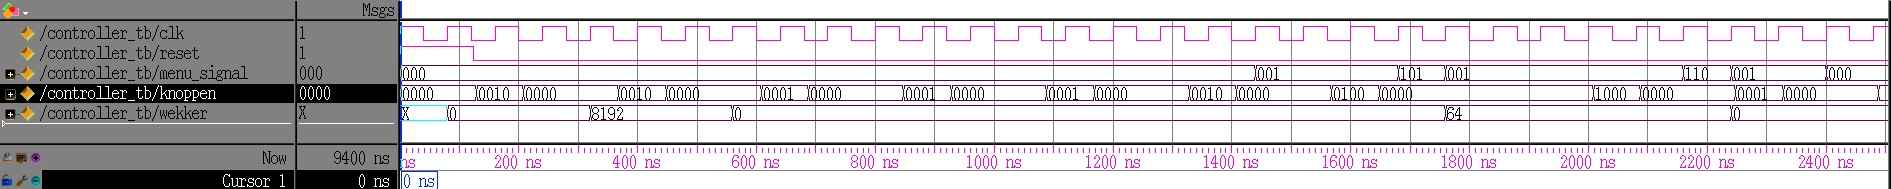
\includegraphics[width=\textwidth,height=\textheight,keepaspectratio]{Figuren/Controller/wave0-2_5_inv.jpg}
\caption{Simulatie van 0 tot 2500ns}
\label{fig:sim_beh_0-2_5}
\end{figure}
\begin{figure}[ht!]
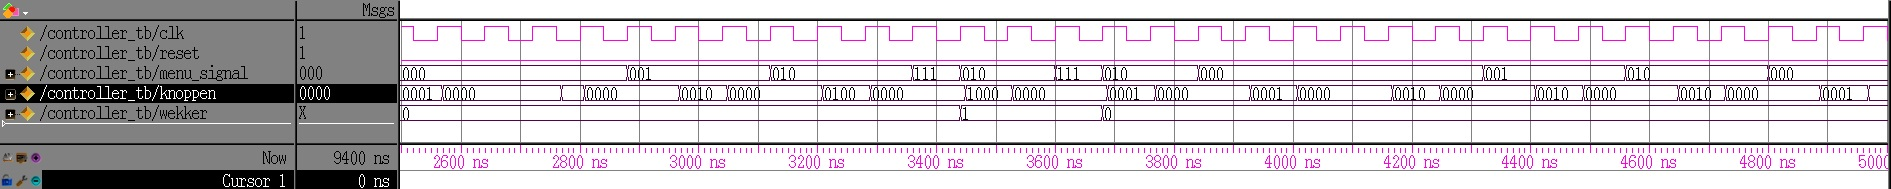
\includegraphics[width=\textwidth,height=\textheight,keepaspectratio]{Figuren/Controller/wave2_5-5_inv.jpg}
\caption{Simulatie van 2500ns tot 5000ns}
\label{fig:sim_beh_2_5-5}
\end{figure}
\begin{figure}[ht!]
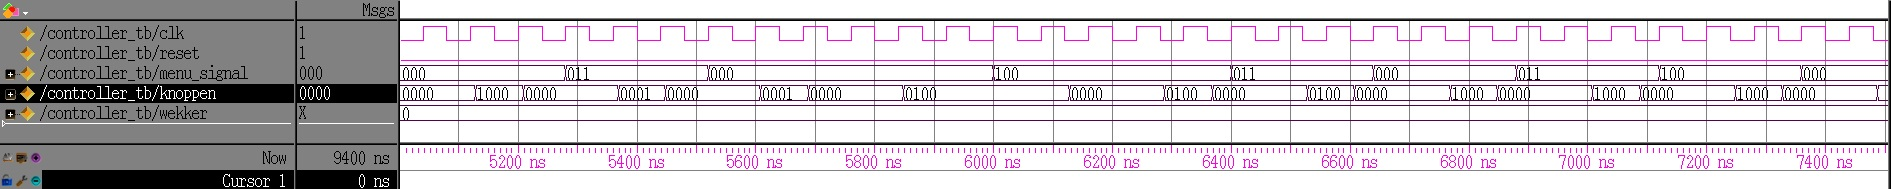
\includegraphics[width=\textwidth,height=\textheight,keepaspectratio]{Figuren/Controller/wave5-7_5_inv.jpg}
\caption{Simulatie van 5000ns tot 7500ns}
\label{fig:sim_beh_5-7_5}
\end{figure}
\begin{figure}[ht!]
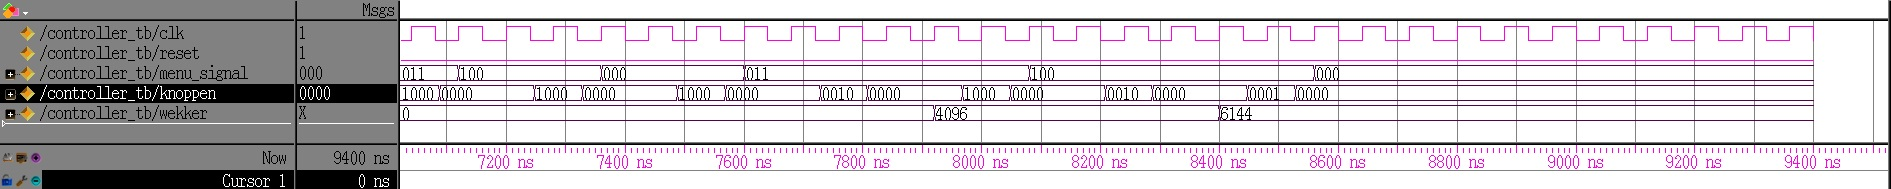
\includegraphics[width=\textwidth,height=\textheight,keepaspectratio]{Figuren/Controller/wave7_5-_inv.jpg}
\caption{Simulatie van 7500ns tot het einde}
\label{fig:sim_beh_7_5-}
\end{figure}
\newpage
\section{Synthesize simulatie}
\begin{figure}[ht!]
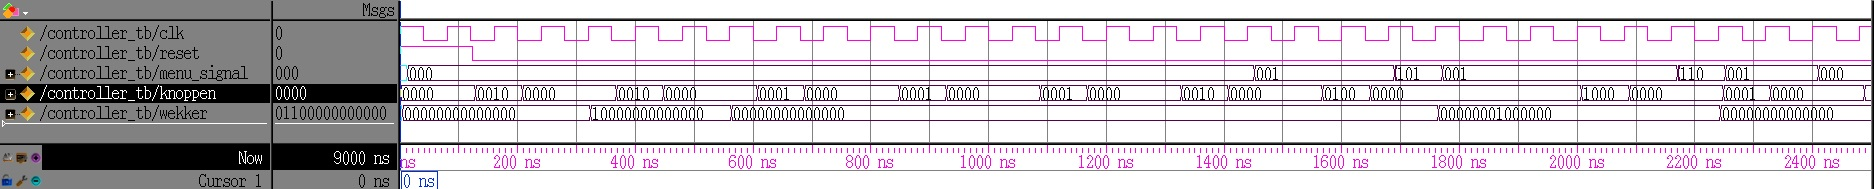
\includegraphics[width=\textwidth,height=\textheight,keepaspectratio]{Figuren/Controller/wave0-2_5_syn_inv.jpg}
\caption{Simulatie van 0 tot 2500ns}
\label{fig:sim_syn_0-2_5}
\end{figure}
\begin{figure}[ht!]
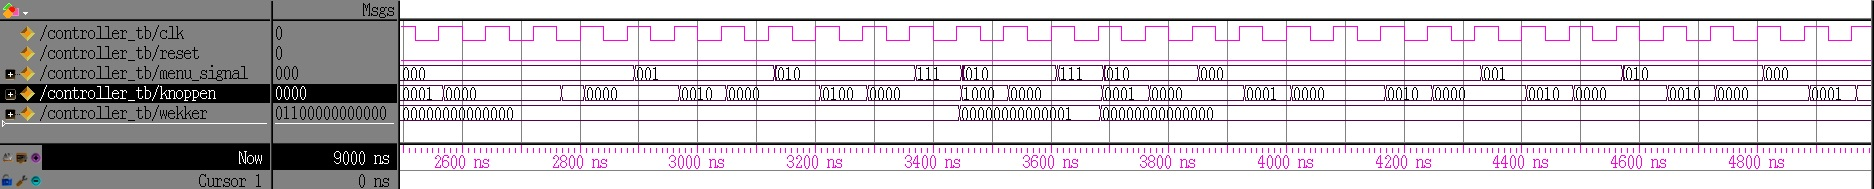
\includegraphics[width=\textwidth,height=\textheight,keepaspectratio]{Figuren/Controller/wave2_5-5_syn_inv.jpg}
\caption{Simulatie van 2500ns tot 5000ns}
\label{fig:sim_syn_2_5-5}
\end{figure}
\begin{figure}[ht!]
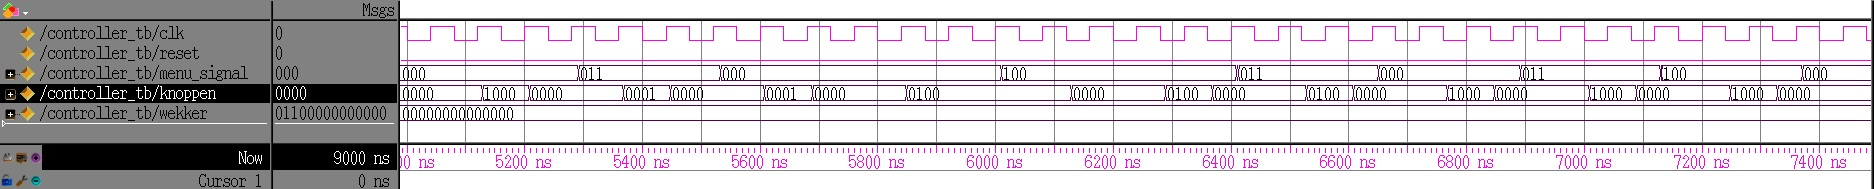
\includegraphics[width=\textwidth,height=\textheight,keepaspectratio]{Figuren/Controller/wave5-7_5_syn_inv.jpg}
\caption{Simulatie van 5000ns tot 7500ns}
\label{fig:sim_syn_5-7_5}
\end{figure}
\begin{figure}[ht!]
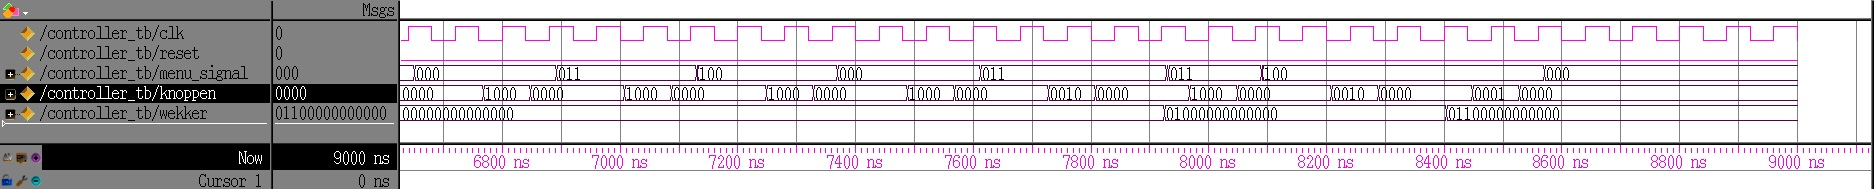
\includegraphics[width=\textwidth,height=\textheight,keepaspectratio]{Figuren/Controller/wave7_5-_syn_inv.jpg}
\caption{Simulatie van 7500ns tot het einde}
\label{fig:sim_syn_7_5-}
\end{figure}
\newpage
\section{Extracted simulatie}
\begin{figure}[ht!]
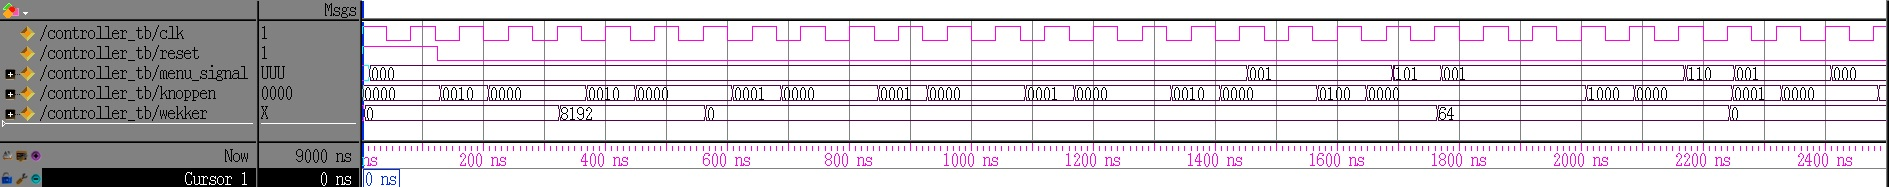
\includegraphics[width=\textwidth,height=\textheight,keepaspectratio]{Figuren/Controller/wave0-2_5_ext_inv.jpg}
\caption{Simulatie van 0 tot 2500ns}
\label{fig:sim_ext_0-2_5}
\end{figure}
\begin{figure}[ht!]
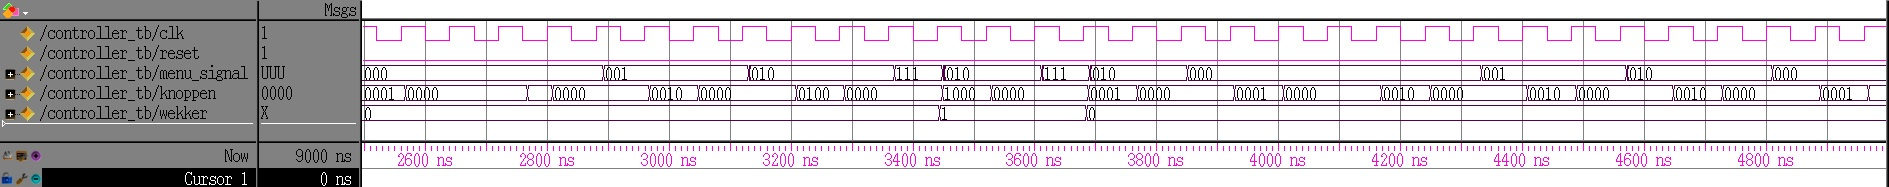
\includegraphics[width=\textwidth,height=\textheight,keepaspectratio]{Figuren/Controller/wave2_5-5_ext_inv.jpg}
\caption{Simulatie van 2500ns tot 5000ns}
\label{fig:sim_ext_2_5-5}
\end{figure}
\begin{figure}[ht!]
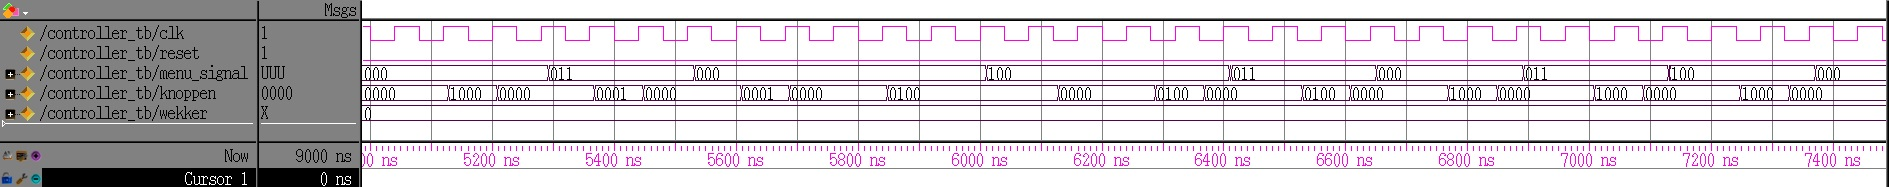
\includegraphics[width=\textwidth,height=\textheight,keepaspectratio]{Figuren/Controller/wave5-7_5_ext_inv.jpg}
\caption{Simulatie van 5000ns tot 7500ns}
\label{fig:sim_ext_5-7_5}
\end{figure}
\begin{figure}[ht!]
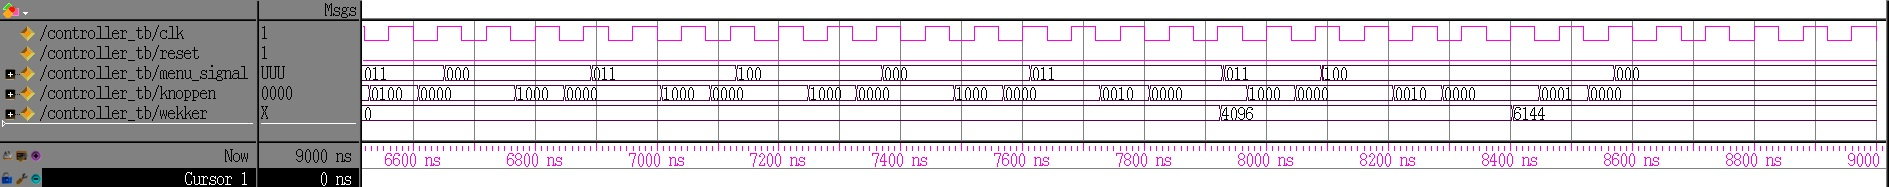
\includegraphics[width=\textwidth,height=\textheight,keepaspectratio]{Figuren/Controller/wave7_5-_ext_inv.jpg}
\caption{Simulatie van 7500ns tot het einde}
\label{fig:sim_ext_7_5-}
\end{figure}
\newpage
\section{Timing}
\begin{figure}[ht!]
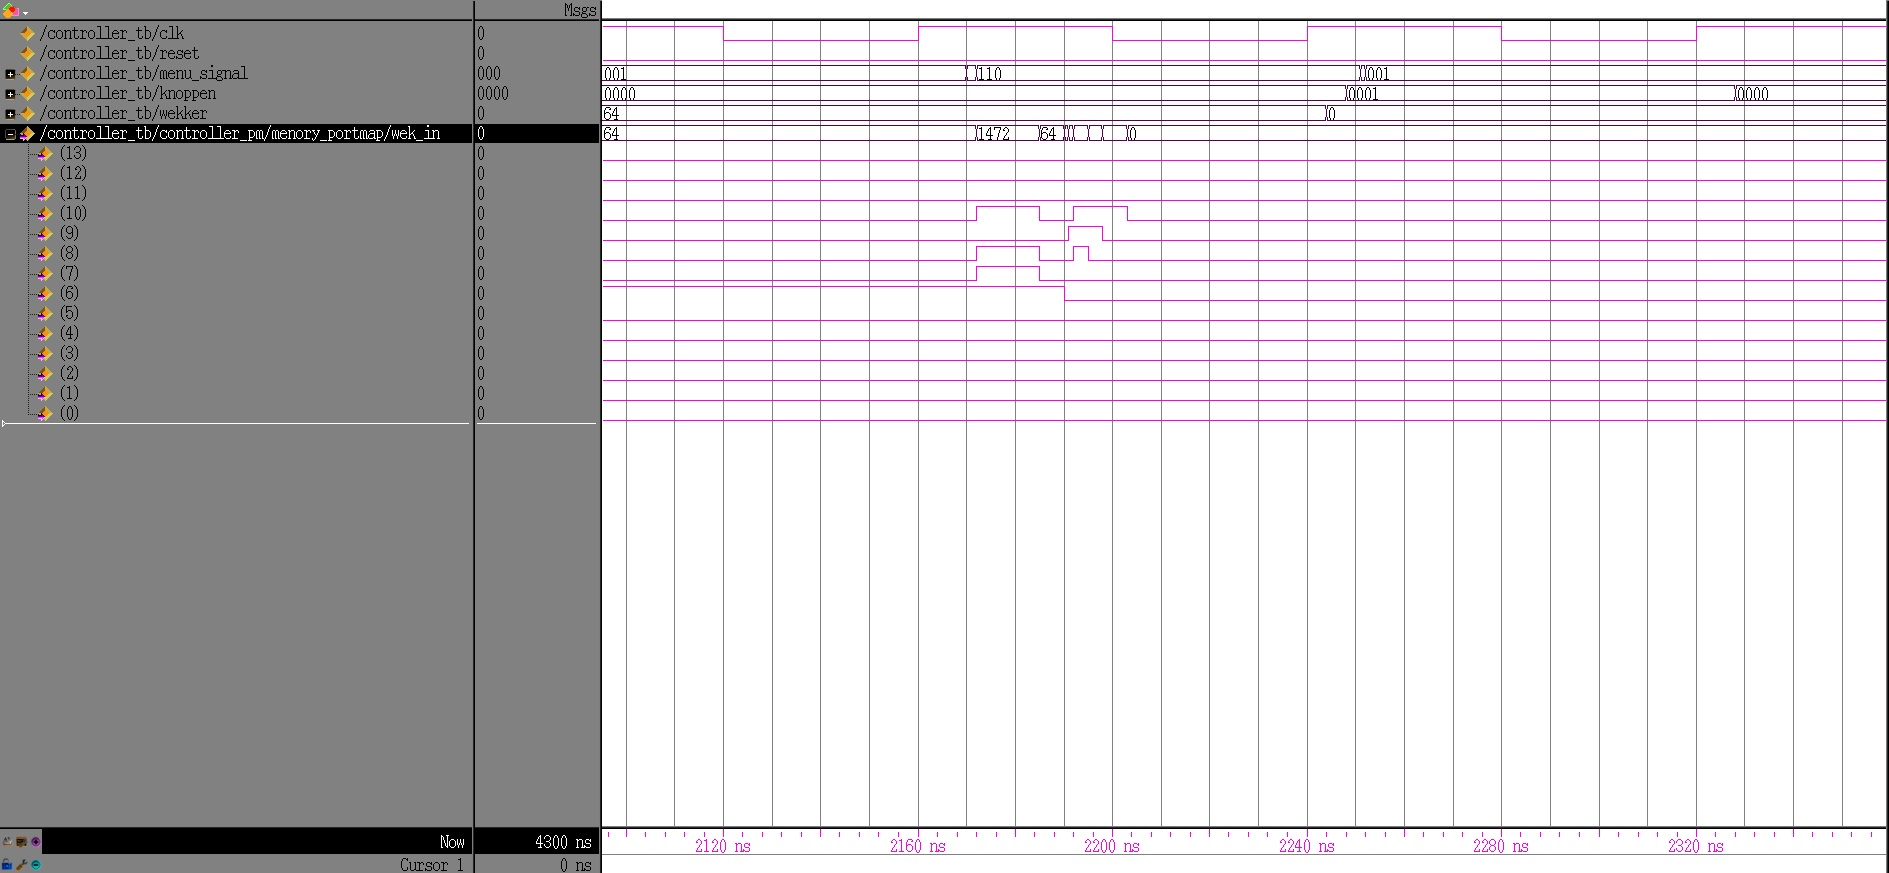
\includegraphics[width=\textwidth,height=\textheight,keepaspectratio]{Figuren/Controller/gliches_min_inv.jpg}
\caption{Timing problemen}
\label{fig:timing_controller}
\end{figure}

\chapter[Simulatie resultaten Alarm]{Simulaties resultaten van het alarm}
\label{Ap:sim_alarm}
\section{Behavioral simulatie}
\begin{figure}[ht!]
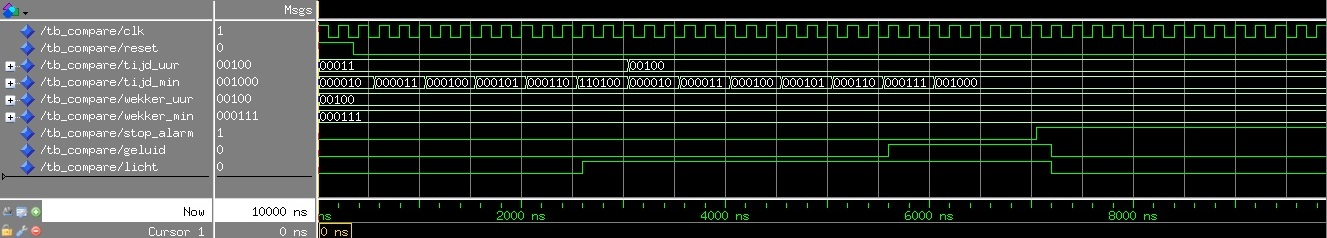
\includegraphics[width=\textwidth,height=\textheight,keepaspectratio]{Figuren/Alarm/Compare_beh.jpg}
\caption{Simulatie van 0 tot 10000 ns van compare}
\label{fig:sim_beh_compare}
\end{figure}
\begin{figure}[ht!]
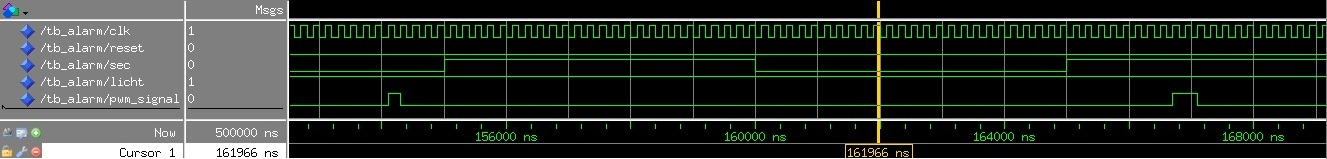
\includegraphics[width=\textwidth,height=\textheight,keepaspectratio]{Figuren/Alarm/Alarm_beh.jpg}
\caption{Simulatie van 151000 tot 170000 ns van alarm}
\label{fig:sim_beh_alarm}
\end{figure}
\newpage
\section{Extracted simulatie}
\begin{figure}[ht!]
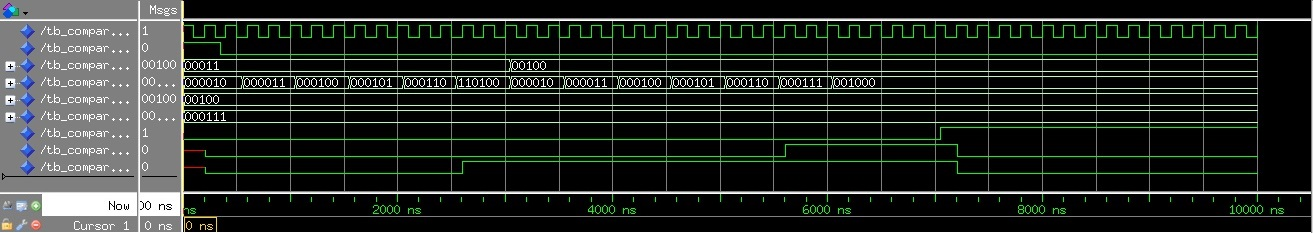
\includegraphics[width=\textwidth,height=\textheight,keepaspectratio]{Figuren/Alarm/Compare_ext.jpg}
\caption{Simulatie van 0 tot 10000 ns van alarm}
\label{fig:sim_ext_compare}
\end{figure}
\begin{figure}[ht!]
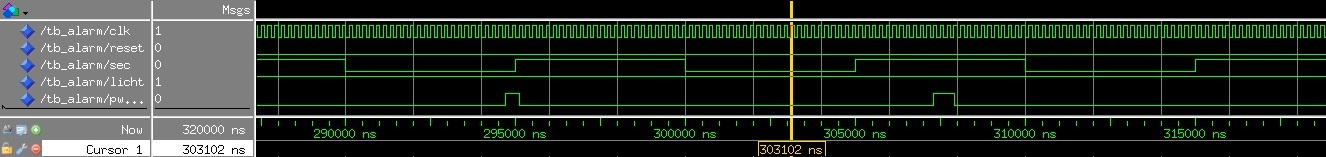
\includegraphics[width=\textwidth,height=\textheight,keepaspectratio]{Figuren/Alarm/Alarm_ext.jpg}
\caption{Simulatie van 290000 tot 320000 ns van alarm}
\label{fig:sim_ext_alarm}
\end{figure}

\chapter[Simulatie resultaten LCD]{Simulaties resultaten van het LCD}
\label{Ap:sim_LCD}
\section{Menu}
\begin{figure}[h!]
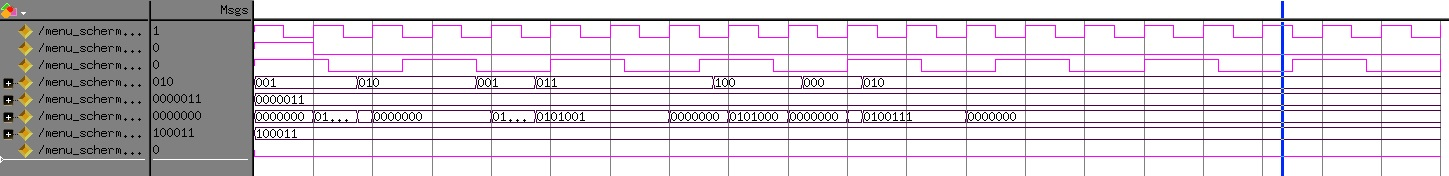
\includegraphics[width=\textwidth,height=\textheight,keepaspectratio]{Figuren/LCD/resultaten/menu.jpg}
\caption{Simulatie van het subblok menu}
\label{fig:simmenu}
\end{figure}
\section{Geluid}
\begin{figure}[h!]
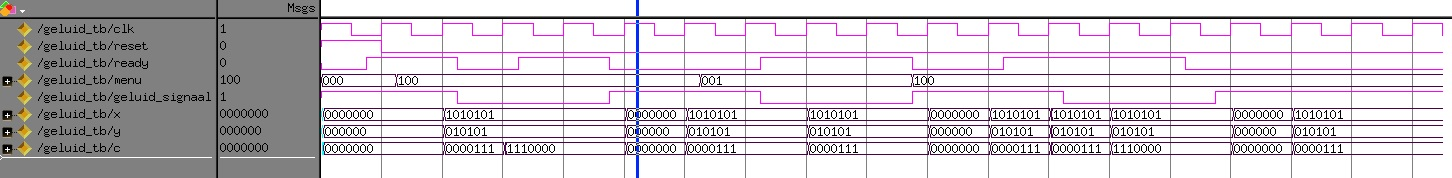
\includegraphics[width=\textwidth,height=\textheight,keepaspectratio]{Figuren/LCD/resultaten/geluid.jpg}
\caption{Simulatie van het subblok geluid}
\label{fig:simgeluid}
\end{figure}
\section{Licht}
\begin{figure}[h!]
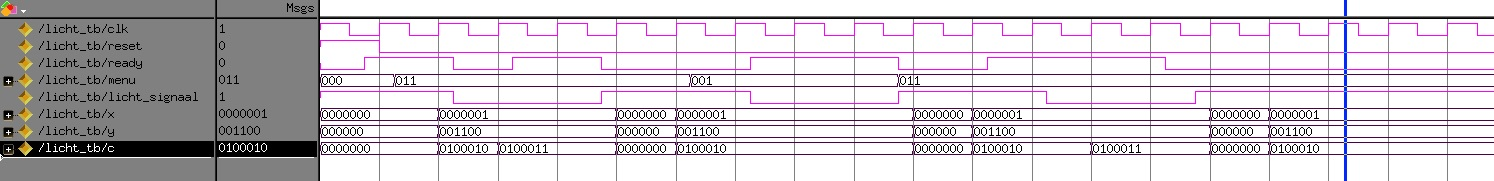
\includegraphics[width=\textwidth,height=\textheight,keepaspectratio]{Figuren/LCD/resultaten/licht.jpg}
\caption{Simulatie van het subblok licht}
\label{fig:simlicht}
\end{figure}
\section{DCF}
\begin{figure}[h!]
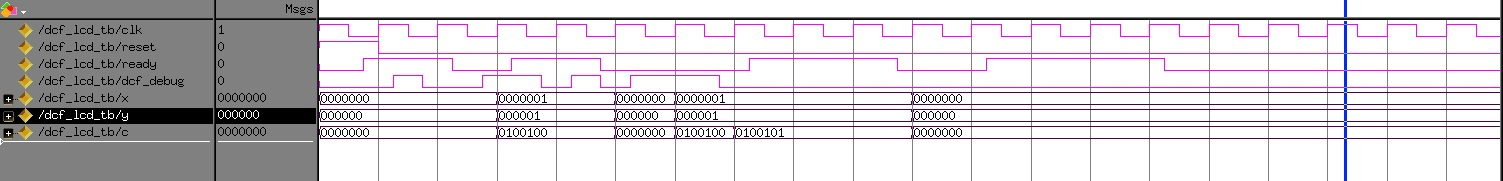
\includegraphics[width=\textwidth,height=\textheight,keepaspectratio]{Figuren/LCD/resultaten/dcf.jpg}
\caption{Simulatie van het subblok dcf}
\label{fig:simdcf}
\end{figure}

\begin{figure}[h!]
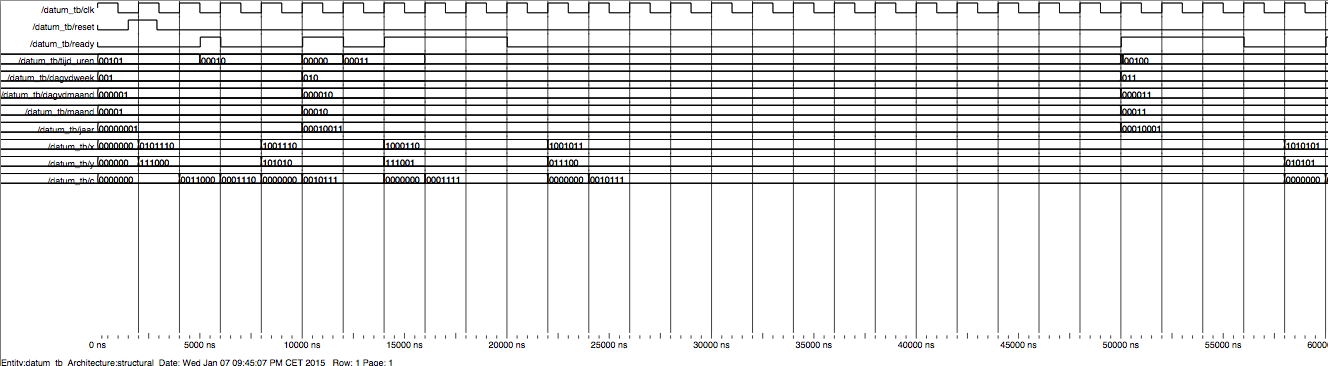
\includegraphics[width=\textwidth,height=\textheight,keepaspectratio]{Figuren/LCD/resultaten/simulatie_datum_behavioural.png}
\caption{Simulatie behavioural van het subblok datum}
\label{fig:sim_datum_behavioural}
\end{figure}

\begin{figure}[h!]
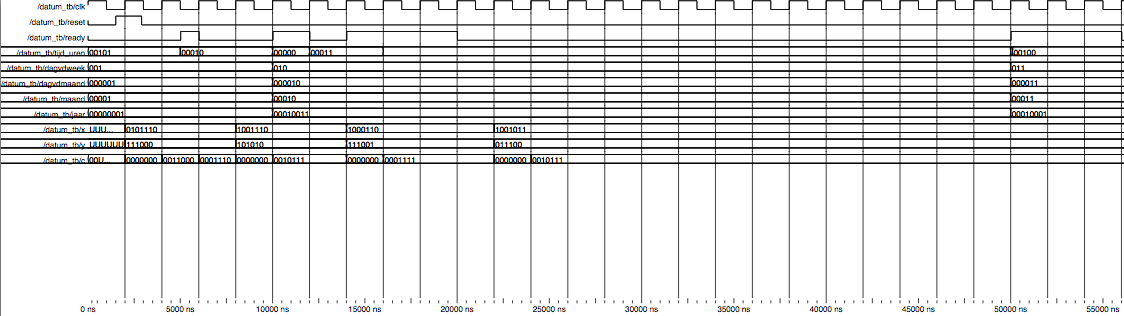
\includegraphics[width=\textwidth,height=\textheight,keepaspectratio]{Figuren/LCD/resultaten/simulatie_datum_circuit.png}
\caption{Simulatie circuit van het subblok datum}
\label{fig:sim_datum_circuit}
\end{figure}

\begin{figure}[h!]
	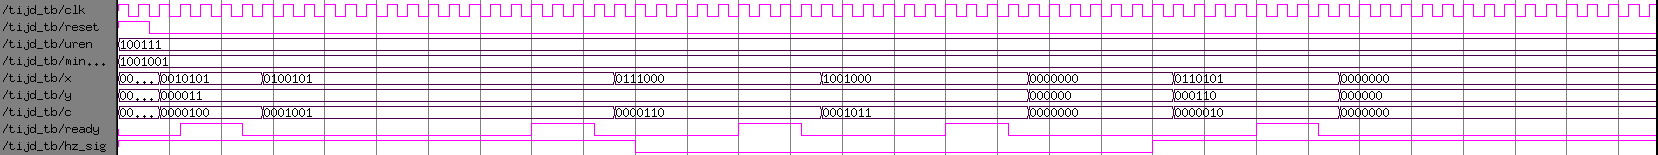
\includegraphics[width=\textwidth,height=\textheight,keepaspectratio]{Figuren/LCD/resultaten/sim_tijd.png}
	\caption{Simulatie van het subblok tijd}
	\label{fig:sim_tijd}
\end{figure}

\begin{figure}[h!]
	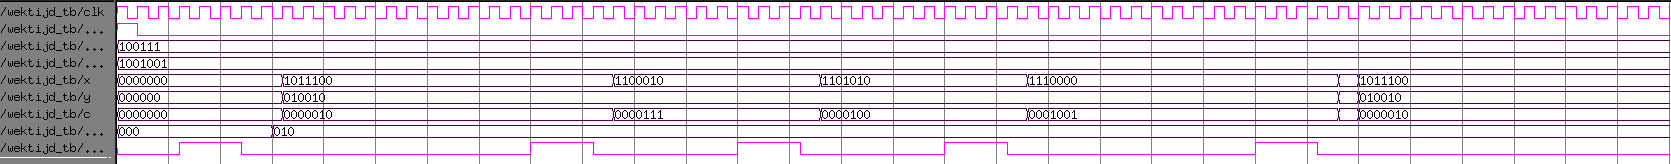
\includegraphics[width=\textwidth,height=\textheight,keepaspectratio]{Figuren/LCD/resultaten/sim_wektijd.png}
	\caption{Simulatie van het subblok wektijd}
	\label{fig:sim_wektijd}
\end{figure}

\begin{figure}[h!]
	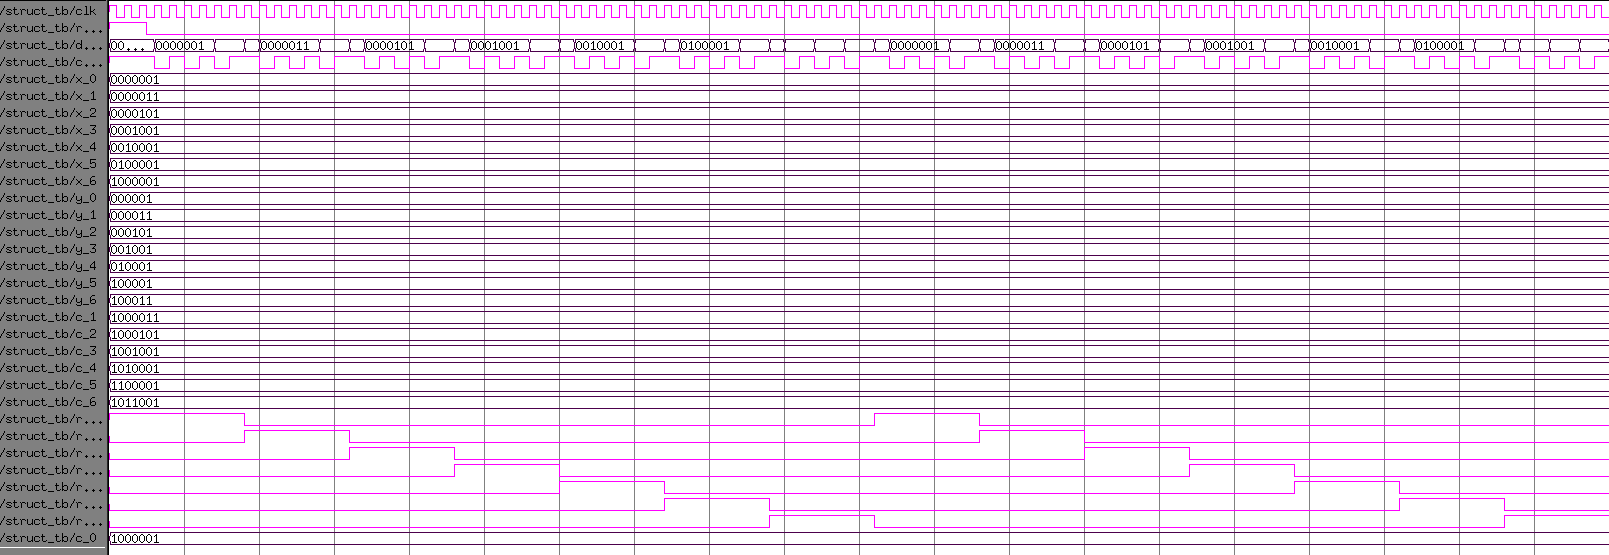
\includegraphics[width=\textwidth,height=\textheight,keepaspectratio]{Figuren/LCD/resultaten/sim_send_top.png}
	\caption{Simulatie van de subblokken send controller en de send bus}
	\label{fig:sim_send_top}
\end{figure}